%%%%%%%%%%%%%%%%%%%%%%%%%%%%%%%%%%%%%%%%%%%%%%%%%%%%%%%%%%%%%%%%%%%%%%%%%%%%%
%集録提出用のサンプルファイルです。
%このファイルを参考にして集録を作成してください。
%%%%%%%%%%%%%%%%%%%%%%%%%%%%%%%%%%%%%%%%%%%%%%%%%%%%%%%%%%%%%%%%%%%%%%%%%%%%%
%%%%%%%%%%%%%%%%%%%%%%%%%%%%%%%%%%%%%%%%%%%%%%%%%%%%%%%%%%%%%%%%%%%%%%%%%%%%%
\documentclass[a4paper,10pt,oneside,twocolumn,notitlepage,final]{jarticle}
\usepackage{ss17(UTF-8)}
%%%%%%%%%%%%%%%%%%%%%%%%%%%%%%%%%%%%%%%%%%%%%%%%%%%%%%%%%%%%%%%%%%%%%%%%%%%%%
%%ss17.styファイルはtexファイルと同じディレクトリに置いてください。
%%ヘッダ、フッターなどの全体のレイアウトは変更しないでください。
%%ここより上は変更しないでください。
%%%%%%%%%%%%%%%%%%%%%%%%%%%%%%%%%%%%%%%%%%%%%%%%%%%%%%%%%%%%%%%%%%%%%%%%%%%%%
%%使いたいパッケージがある場合は以下に書いてください。
\usepackage[dvipdfmx]{graphicx,color} 


%%%%%%%%%%%%%%%%%%%%%%%%%%%%%%%%%%%%%%%%%%%%%%%%%%%%%%%%%%%%%%%%%%%%%%%%%%%%%
%%名前、所属、タイトルは以下に記入してください。
%%所属は以下のように()内にお願いします。
\author{磯谷 和秀 (名古屋大学大学院 理学研究科)}
\title{巨大衝突ステージにおける衝突破壊の重要性:\\
$N$体計算$\cdot$統計的手法のハイブリッドコードの開発}
%%%%%%%%%%%%%%%%%%%%%%%%%%%%%%%%%%%%%%%%%%%%%%%%%%%%%%%%%%%%%%%%%%%%%%%%%%%%%


\begin{document}


%%概要は\abst内に記入してください。
%%\maketitleは必要ありません。
%%以下の\abst{}に概要を記入することにより
%%タイトル、名前、日付、概要が一括して出力されます。
\abst{
太陽系の地球型惑星は、最終段階で火星サイズの原始惑星同士が衝突合体を繰り返し形成される。この巨大衝突ステージにおいて地球や地球-月系が形成される。
一方、太陽系外で起こる巨大衝突ステージは、衝突に伴い放出される破片によりデブリ円盤が形成され、観測されている暖かいデブリ円盤(すなわち地球形成領域のデブリ円盤)を説明することができる。
巨大衝突ステージに形成されるデブリ円盤について調べるためには、原始惑星の長期的軌道進化と、破壊を扱うことができる計算が必要である。
そこで本研究では、$N$体計算と統計的手法を組み合わせた、衝突破壊を扱うことができるハイブリッドコードの開発を行う。
さらに本講演では、ハイブリッドコードにより得られる、巨大衝突ステージにおけるデブリ円盤の明るさの空間分布進化についても議論する。
}



\section{Introduction}
太陽系の地球型惑星は、大きく分けて3つのステージを経て形成される。
まずダストから微惑星が形成、次に微惑星から原始惑星が形成、そして最後に原始惑星から地球型惑星が形成される。
この最後の巨大衝突ステージでは原始惑星同士が衝突合体を繰り返しているが、衝突が起きれば自然に破壊も起こり、様々なサイズの破片を放出することがSPH法によるシミュレーションで明らかになった\citep[e.g.,][]{Genda2015}。
この原始惑星同士の巨大衝突による破片が、太陽系外の$10^6 - 10^7$歳程度以上の星の周りで観測されている暖かい($\lesssim 1 {\rm AU}$)デブリ円盤の起源なのではないかと言われている\citep[e.g.,][]{Lisse2008,Lisse2009}。
またさらに、$N$体計算によって明らかになった、衝突合体を繰り返した原始惑星の軌道離心率や軌道傾斜角が大きくなりすぎてしまう問題\citep{Kokubo2006}は、デブリ円盤中の破片による力学的摩擦が働くことで解決できるかもしれない\citep[e.g.,][]{O'Brien2006}。
このように、巨大衝突ステージにおける衝突破壊は重要であり、また実験室でこの規模の衝突を再現することは困難であるため、この現象を理解するためには、原始惑星の長期的軌道進化と破壊を扱うことができる数値シミュレーションが必要である。
しかし衝突により放出される破片の数は$10^{35}$個以上にもなり、$N$体計算ではとても扱うことはできない。
このような多数の粒子を取り扱うには、一つ一つの粒子を取り扱うのではなく、統計力学に基づいた統計的手法が有効であるが、統計的手法では、破片が重力的に集積する際にサイズ分布が非軸対称になることや、原始惑星による軌道共鳴のような、重力相互作用の取り扱いができない。
すなわち$N$体計算と統計的手法を同時に用いると、軌道進化と破壊を同時に考慮した計算を行うことができる。

そこで本研究では、$N$体計算と統計的手法を組み合わせた、衝突破壊を扱うことができるハイブリッドコードの開発を行う。
多数の破片を少数のトレーサーと呼ばれるスーパー粒子に近似することで$N$体計算のコストを抑える。
またそれぞれのトレーサーの周りに扇形領域\citep{Morishima2015}を考え、その領域に入った他のトレーサーを用いて表面数密度と平均相対速度を計算し、破壊による天体の減少\citep{Kobayashi2010}を取り扱う。


\section{Methods}

\subsection{$N$体計算}
本研究では、以下で述べる4次のエルミート法\citep{Makino1992}用いて重力相互作用を取り扱い、さらに独立タイムステップを採用する。

時間$t$での位置と速度(${\bm x}_{0,j},{\bm v}_{0,j}$)、加速度とその時間微分(${\bm a}_{0,j},\dot{{\bm a}}_{0,j}$)から、時間$t + \Delta t$における位置と速度(${\bm x}_{p,j} , {\bm v}_{p,j}$)を次のように予測する。
\begin{align}
{\bm x}_{p,j} &= {\bm x}_{0,j} + \Delta t {\bm v}_{0,j} + \frac{\Delta t ^2}{2} {\bm a}_{0,j} + \frac{\Delta t ^3}{6} \dot{{\bm a}}_{0,j}\\
{\bm v}_{p,j} &= {\bm v}_{0,j} + \Delta t {\bm a}_{0,j} + \frac{\Delta t ^2}{2} \dot{{\bm a}}_{0,j}
\end{align}
これらを予測子と呼ぶ。この段階では2次精度である。
次に予測子を使って, 時間$t + \Delta t$での加速度とその時間微分(${\bm a}_{1,j},\dot{{\bm a}}_{1,j}$)を次のように求める.
\begin{align}
{\bm a}_{1,j} &= - \sum_{k \not= j} G m_k \frac{{\bm r}_{jk}}{(r_{jk}^2 + \epsilon^2)^{3/2}}\label{eq:a1j}\\
\dot{{\bm a}}_{1,j} &= - \sum_{k \not= j} G m_k \left[ \frac{{\bm v}_{jk}}{(r_{jk}^2 + \epsilon^2)^{3/2}} - \frac{3 ( {\bm v}_{jk} \cdot {\bm r}_{jk} ) {\bm r}_{jk} }{(r_{jk}^2 + \epsilon^2)^{5/2}} \right]\label{eq:adot1j}
\end{align}
ここで,
\begin{align}
{\bm r}_{jk} &= {\bm x}_{p,j} - {\bm x}_{p,k}\\
{\bm v}_{jk} &= {\bm v}_{p,j} - {\bm v}_{p,k} 
\end{align}
であり、$\epsilon$は計算上の発散を抑えるためのソフトニングパラメータである(本研究では$\epsilon=0$)。
続いて、時間$t$から$t+\Delta t$間の加速度の時間変化を
\begin{align}
{\bm a}_{1,j} &= {\bm a}_{0,j} + \Delta t \dot{{\bm a}}_{0,j} + \frac{\Delta t ^2}{2} {\bm a}_{0,j}^{(2)} + \frac{\Delta t ^3}{6} {\bm a}_{0,j}^{(3)}\\
\dot{{\bm a}}_{1,j} &= \dot{{\bm a}}_{0,j} + \Delta t {\bm a}_{0,j}^{(2)} + \frac{\Delta t ^2}{2} {\bm a}_{0,j}^{(3)}
\end{align}
のような3次の補間多項式で近似する。
ここで、${\bm a}_{0,j}^{(2)},{\bm a}_{0,j}^{(3)}$は時間$t$における加速度の2階と3階の時間導関数であり、エルミート補間より
\begin{align}
{\bm a}_{0,j}^{(2)} &= \frac{- 6 ({\bm a}_{0,j} - {\bm a}_{1,j}) - \Delta t (4 \dot{{\bm a}}_{0,j} + 2 \dot{{\bm a}}_{1,j})}{\Delta t ^2}\\
{\bm a}_{0,j}^{(3)} &= \frac{12 ({\bm a}_{0,j} - {\bm a}_{1,j}) + 6 \Delta t (\dot{{\bm a}}_{0,j} + \dot{{\bm a}}_{1,j})}{\Delta t ^3}
\end{align}
となる。
そして、この${\bm a}_{0,j}^{(2)},{\bm a}_{0,j}^{(3)}$を使って,位置と速度の予測子を以下のように修正する.
\begin{align}
{\bm x}_{c,j} &= {\bm x}_{p,j} + \frac{\Delta t ^4}{24} {\bm a}_{0,j}^{(2)} + \frac{\Delta t ^5}{120} {\bm a}_{0,j}^{(3)}\\
{\bm v}_{c,j} &= {\bm v}_{p,j} + \frac{\Delta t ^3}{6} {\bm a}_{0,j}^{(2)} + \frac{\Delta t ^4}{24} {\bm a}_{0,j}^{(3)}
\end{align}
これらを修正子と呼ぶ。
修正子を使って新たな加速度とその時間微分(${\bm a}_{1,j}^{\rm new},\dot{{\bm a}}_{1,j}^{\rm new}$)を計算する.これらは,式(\ref{eq:a1j}),式(\ref{eq:adot1j})で,
\begin{align}
{\bm r}_{jk} &= {\bm x}_{c,j} - {\bm x}_{c,k}\\
{\bm v}_{jk} &= {\bm v}_{c,j} - {\bm v}_{c,k} 
\end{align}
とすれば求まる.必要な回数だけ修正を繰り返す。最後の${\bm a}_{1,j}^{\rm new},\dot{{\bm a}}_{1,j}^{\rm new}$を次のステップのための${\bm a}_{0,j},\dot{{\bm a}}_{0,j}$に更新する.

独立タイムステップでは、粒子$j$ごとに別々の時間$t_j$とタイムステップ$\Delta t_j$をもち、別々に時間発展する。
まず、タイムステップの計算には以下の表式を用いる\citep{Aarseth1985}。
\begin{align}
\Delta t_j = \sqrt{\eta \frac{| {\bm a}_{1,j}| | {\bm a}_{1,j}^{(2)} | + | \dot{{\bm a}}_{1,j}| ^2}{| \dot{{\bm a}}_{1,j}| | {\bm a}_{1,j}^{(3)} | + | {\bm a}_{1,j}^{(2)} | ^2}}
\end{align}
これは4次スキームでは非常に効率が良いことが分かっている\citep{Makino1991}。ここで、$\eta$は積分の精度を決めるパラメータである。また${\bm a}_{1,j}^{(2)} = {\bm a}_{0,j}^{(2)} + {\bm a}_{0,j}^{(3)} \Delta t, {\bm a}_{1,j}^{(3)} = {\bm a}_{0,j}^{(3)}$と見積もる。
系全体の時間$t_{\rm sys}$は、$t_j + \Delta t_j$が最小になる粒子$j_{\rm sys}$と共に進める。そして$t_{\rm sys}$における全ての予測子を計算し、$j_{\rm sys}$のみ修正をし、$t_{j_{\rm sys}}$のみ$\Delta t_{j_{\rm sys}}$だけ時間を進める。これを繰り返して時間発展させる。

\subsection{統計的手法}
衝突破壊の際に放出される破片の数は$10^{35}$個以上にもなり、個々の破片を$N$体計算で扱うことは計算コスト的に非常に困難である。そこで本研究では、ほぼ同じ軌道上を運動する複数の破片を1つの粒子(トレーサーと呼ぶ)として表現するスーパー粒子近似を用いる。また、破片同士の破壊が次々に起こり「衝突カスケード」が形成されると、定常な負の質量フラックスが生まれる\citep{Tanaka1996}。質量フラックスと質量減少タイムスケールについての解析解\citep{Kobayashi2010}と、トレーサーの周囲に扇形領域\citep{Morishima2015}を形成し、その領域内で面密度と平均相対速度を求めることにより、$\mu {\rm m}$サイズとなった破片がどの程度トレーサーから出て行くかを計算することができる。以下で詳しく説明する。

トレーサーの中には様々な質量をもった破片が存在し、質量$m$から$m+dm$の範囲における破片の質量分布$n(m)dm$が
\begin{align}
 n(m)dm = m^{-b}dm
\end{align}
のようにべき$b$(無次元パラメータ)で表現でき、破片の面数密度$n_{\rm s} (m) dm$が
\begin{align}
 n_{\rm s} (m) dm = A m^{- \alpha} dm
\end{align}
のように係数$A$とべき$\alpha$(無次元パラメータ)で表現できると仮定する。さらに$m$を横切る質量フラックスを$F(m)$とおく。また、衝突される天体の質量$m_1$、1回の衝突で放出された破片の総質量$m_{\rm e}$、そして1回の衝突で放出された破片の最大質量$m_{\rm L}$の関係が、
\begin{align}
 m_{\rm e} &= \frac{\phi}{1 + \phi}m_1\\
 m_{\rm L} &= \frac{\epsilon}{1 + \phi}m_{\rm e} = \frac{\epsilon \phi}{(1 + \phi)^2}m_1
\end{align}
のように与えられるモデルを使う。ここで、係数$\epsilon$は無次元パラメータである。これらは臨界エネルギー$Q_{\rm D}^{\ast}$で規格化した衝突エネルギー$\phi$のみの関数となっている。衝突する天体の質量$m_2$、$m_1$と$m_2$の衝突速度$v$を用いると、
\begin{align}
 \phi = \frac{v^2}{2 Q_{\rm D}^{\ast}} \frac{m_2/m_1}{1 + m_2/m_1}
\end{align}
のように定義される。

$v^2/Q_{\rm D}^{\ast}$が質量に依存しないとき、すなわち破壊のモデルが自己相似の場合、$F(m)$が定常となる条件は
\begin{align}
 \alpha = \frac{11}{6}
\end{align}
である\citep{Tanaka1996}。
一方、$v(m)^2/Q_{\rm D}^{\ast}(m) \propto m^p$のように質量に依存するとき、すなわち破壊のモデルが非自己相似の場合、$F(m)$が定常となる条件は
\begin{align}
 \alpha = \frac{11 + 3p}{6 + 3p}
\end{align}
である\citep{Kobayashi2010}。本研究では非自己相似のときの計算を取り扱う。
破片の最大質量を$m_{\rm max}$、最小質量を$m_{\rm min}$とおくと、$F(m)$が定常ということは$F(m_{\rm min}) = F(m_{\rm max})$である。すなわちトレーサー内の質量減少を$F(m_{\rm max})$で計算することができる。質量フラックスの解析解は
\begin{align}
 F(m_{\rm max}) =& - \frac{(2 - \alpha)^2}{m_{\rm max}^{1/3}} \Sigma^2 \Omega_{\rm K} h_0 \left( \frac{v(m_{\rm max})^2}{Q_{\rm D}^{\ast}(m_{\rm max})} \right)^{\alpha - 1} \nonumber \\
 &\times \left[ \left( - \ln \epsilon + \frac{1}{2 - b} \right) s_1 + s_2 + s_3 \right]
\end{align}
で与えられ、質量減少タイムスケール$\tau_{\rm dep}$は
\begin{align}
 \tau_{\rm dep} = \frac{\Sigma}{|F(m_{\rm max})|}
\end{align}
で与えられる。質量フラックスを計算するためには、トレーサーの面密度と衝突速度を求める必要がある。そこで、まずトレーサー$i$の位置を2次元極座標($r_i,\theta_i$)に射影し、動径方向に$r_i \pm \delta r$、方位角方向に$\theta_i \pm \delta \theta$の広がりをもった扇形領域$i$を形成する。この領域$i$に入っている他のトレーサーを$j$とし、$j$の総数を$N$とする。面密度は$i$自身と$j$の質量の総和を領域$i$の面積で割り、
\begin{align}
 \Sigma_i = \frac{m_i + \sum_{j}^{N} m_j}{4 r_i \delta r \delta \theta}
\end{align}
のように計算する。次にトレーサー$i$と$j$の相対速度は、ランダム速度$\sqrt{e_{i,j}^2 + i_{i,j}^2} v_{{\rm K},i}$で近似する。ここで、$e_{i,j}$と$i_{i,j}$はそれぞれ相対離心率と相対軌道傾斜角を表し、
\begin{align}
 e_{i,j}^2 &= e_i^2 + e_j^2 - 2 e_i e_j \cos(\varpi_i - \varpi_j)\\
 i_{i,j}^2 &= i_i^2 + i_j^2 - 2 i_i i_j \cos(\Omega_i - \Omega_j)
\end{align}
のように定義される。ここで、$\varpi$は近点経度、$\Omega$は昇交点経度である。そして$j$について平均をとり、平均相対速度を衝突速度だとみなす。
\begin{align}
 v_i = \frac{\sum_{j}^{N} \sqrt{e_{i,j}^2+i_{i,j}^2} v_{{\rm K},i}}{N}
\end{align}
以上より質量フラックスを各トレーサーごとに求めることができる。

統計的手法のタイムステップ$\Delta t_{{\rm frag},i}$は質量減少タイムスケール$\tau_{{\rm dep},i}$を基準にして、$\Delta t_{{\rm frag},i} = \xi \tau_{{\rm dep},i}$とする。そしてトレーサー$i$の質量変化は、
\begin{align}
 m_i(t_{{\rm frag},i} + \Delta t_{{\rm frag},i}) = \frac{m_i(t_{{\rm frag},i})}{1 + \xi}
\end{align}
のように計算する。$N$体計算では独立タイムステップを用いているため、トレーサー$i$の$N$体計算の時間$t_i$が統計的手法の時間$t_{{\rm frag},i}$を上回ったときにトレーサー$i$の質量を減少させ、$t_{{\rm frag},i} \to t_{{\rm frag},i} + \Delta t_{{\rm frag},i}$に更新する。




\section{Numerical Test}

\subsection{$N$体計算のテスト}

小さい微惑星と大きい微惑星が混在するときの離心率$\cdot$軌道傾斜角の二乗平均平方根の時間進化.太陽から $1 {\rm AU}$ の位置に質量 $1 \times 10^{24} {\rm g}$ の微惑星を $800$ 個,$4 \times 10^{24} {\rm g}$ の微惑星を $200$ 個配置し,$1000$ 年分計算を6回行った.ここで,初期の微惑星の面密度が $10 {\rm g/cm^2}$ となるように,$0.943 - 1.057 {\rm AU}$ に一様に配置した.また,初期の離心率$\cdot$軌道傾斜角はレイリー分布に従い,それぞれの二乗平均平方根は $e_{\rm RMS} = 1 \times 10^{-4}, i_{\rm RMS} = 5 \times 10^{-5}$ とした.\cite{Ohtsuki2002}のFig.4bとの比較.
\begin{figure}[h]
 \centering
 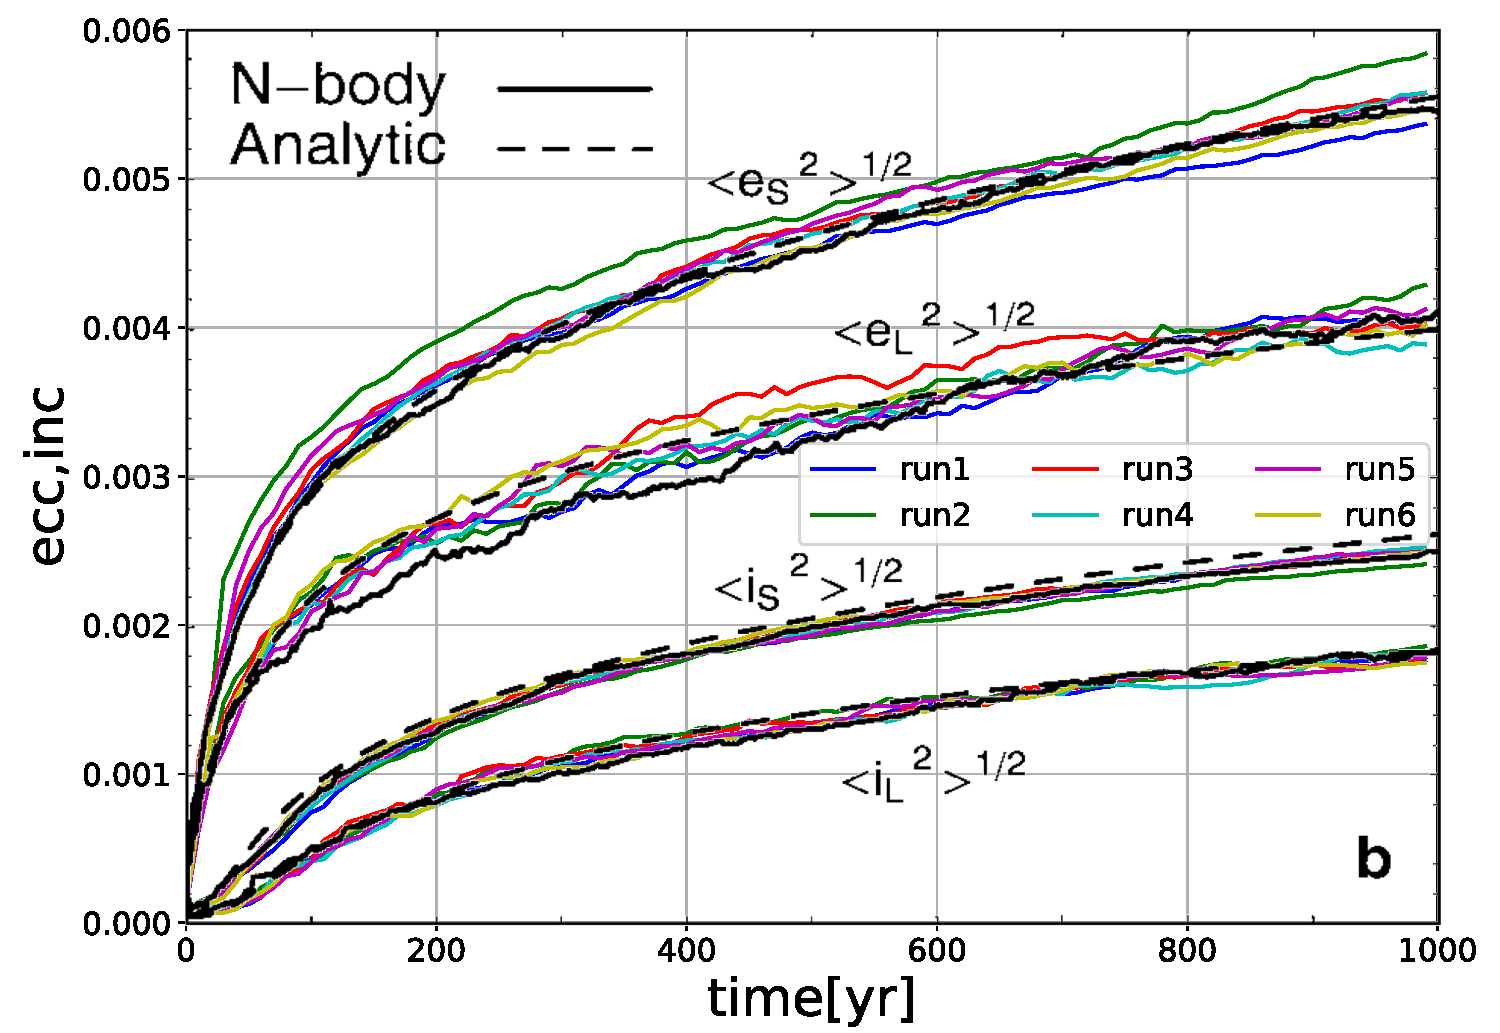
\includegraphics[width=8cm]{Ohtsuki_figb_and_Nbodytest_6run.pdf}
 \caption{\label{}}
\end{figure}

\subsection{統計的手法のテスト}

統計的手法を用いたときの微惑星総質量の時間進化.扇形領域の大きさを決める $\Delta r$ を,$0.01 {\rm AU}$ で固定している.太陽から $0.95 - 1.05 {\rm AU}$ の位置に等質量のトレーサーを $990$ 個一様に配置し,$10^4$ 年分計算を行った.ここで,トレーサー同士の相互重力は計算しておらず,トレーサーの軌道要素は変化していない.すべてのトレーサーは初期に離心率 $e = 10^{-3}$,軌道傾斜角 $i = 5 \times 10^{-4}$ をもち,その他の角変数は等間隔で与えた.質量減少タイムスケール $\tau$ が $10$ 年となるように,初期の総質量を $3.51 \times 10^{30} {\rm g}$ とし,解析解の表式\citep{Kobayashi2010}と比較した.質量減少タイムスケール $\tau$ に対して、実際の統計的計算ではタイムステップを $\xi \tau$ としている.

\begin{figure}[h]
 \centering
 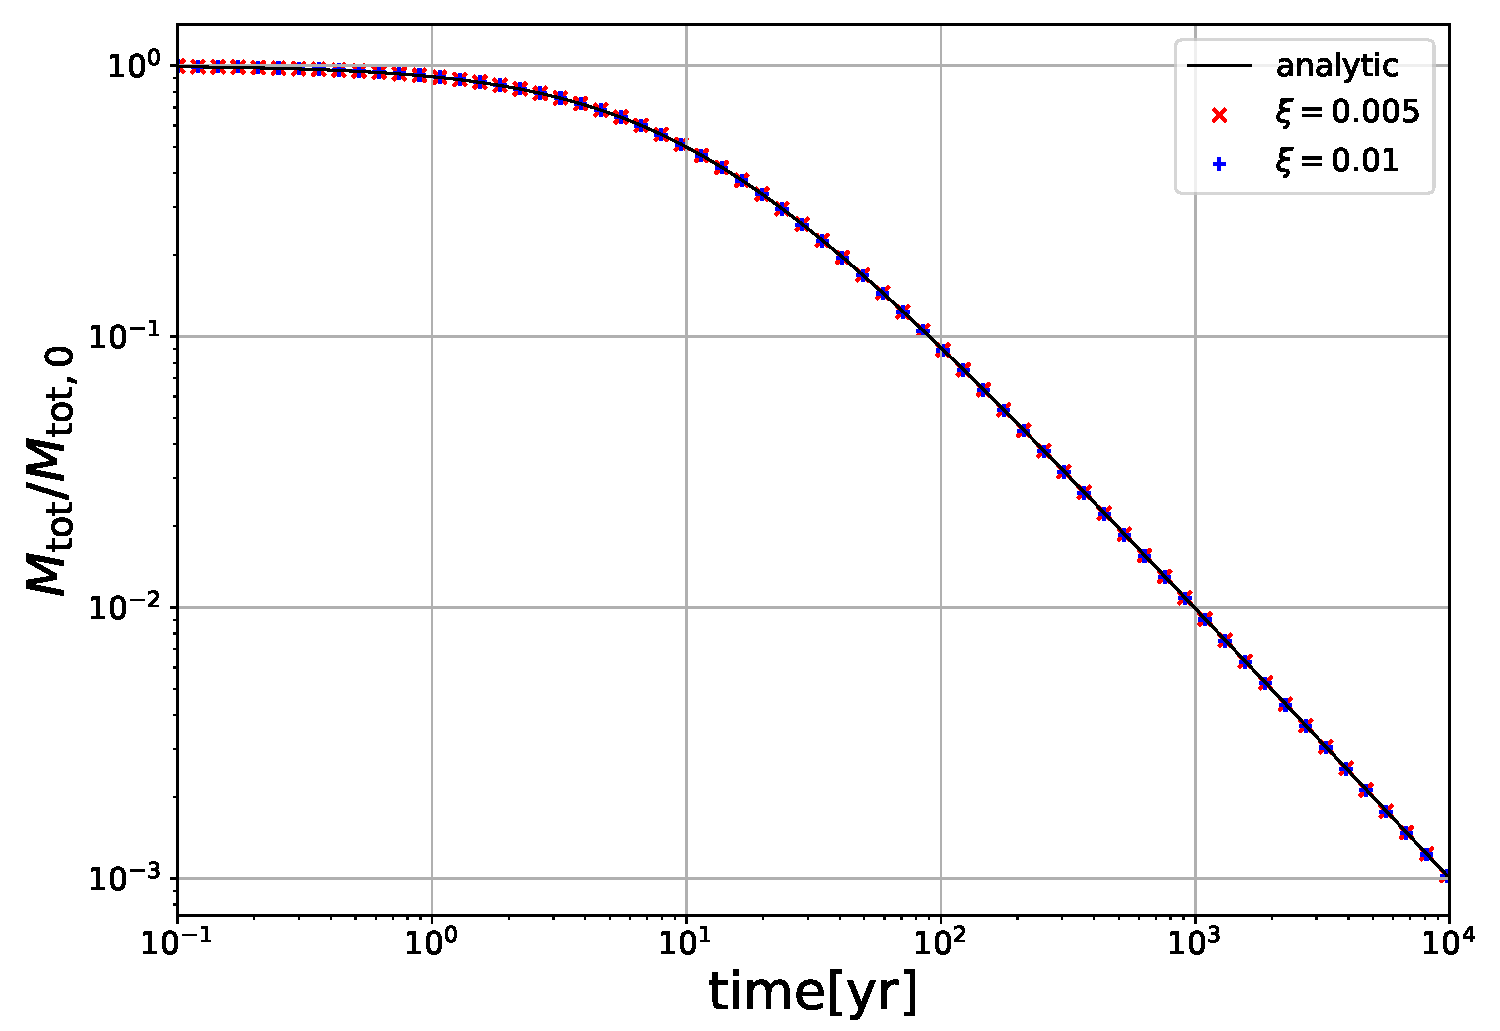
\includegraphics[width=8cm]{MassDepletion.pdf}
 \caption{\label{}}
\end{figure}

\section{Discussion}
本文を記入してください。本文を記入してください。本文を記入してください。本文を記入してください。本文を記入してください。本文を記入してください。


\section{Conclusion}
本文を記入してください。本文を記入してください。本文を記入してください。本文を記入してください。本文を記入してください。本文を記入してください。



\section*{Acknowledgement}
謝辞がある場合は記入してください。

\small
\begin{thebibliography}{99}
 \bibitem[Aarseth(1985)]{Aarseth1985}
 Aarseth, S. J. 1985, in Multiple Time Scales, ed. J. U. Brackbill and B. I. Cohen (New York:Academic), 377
 \bibitem[Genda et al.(2015)]{Genda2015}
 Genda, H., Kobayashi, H., \& Kokubo, E. 2015, ApJ, 810, 136
 \bibitem[Kobayashi \& Tanaka(2010)]{Kobayashi2010}
 Kobayashi, H., \& Tanaka, H. 2010, Icarus, 206, 735
 \bibitem[Kokubo et al.(2006)]{Kokubo2006}
 Kokubo, E., Kominami, J., \& Ida, S. 2006, ApJ, 642, 1131
 \bibitem[Lisse et al.(2008)]{Lisse2008}
 Lisse, C. M., Chen, C. H., Wyatt, M. C. \& Morlok, A. 2008, ApJ, 673, 1106
 \bibitem[Lisse et al.(2009)]{Lisse2009}
 Lisse, C. M., Chen, C. H., Wyatt, M. C., Morlok, A., Song, I., Bryden, G. \& Sheeham, P. 2009, ApJ, 791, 2019
 \bibitem[Makino(1991)]{Makino1991}
 Makino, J. 1991, ApJ, 369, 200
 \bibitem[Makino \& Aarseth(1992)]{Makino1992}
 Makino, J., \& Aarseth, S. J. 1992, PASJ, 44, 141
 \bibitem[Morishima(2015)]{Morishima2015}
 Morishima, R. 2015, Icarus, 260, 368
 \bibitem[O'Brien et al.(2006)]{O'Brien2006}
 O'Brien, D. P., Morbidelli, A., \& Levison, H. F. 2006, Icarus, 184, 39
 \bibitem[Ohtsuki et al.(2002)]{Ohtsuki2002}
 Ohtsuki, K., Stewart, G. R., \& Ida, S. 2002, Icarus, 155, 436
 \bibitem[Tanaka et al.(1996)]{Tanaka1996}
 Tanaka, H., Inaba, S., Nakazawa, K. 1996, Icarus, 123, 450
\end{thebibliography}






\end{document}
